\documentclass[10pt]{extarticle}
\usepackage[utf8]{inputenc}

\usepackage{extsizes}

\usepackage{url}
\usepackage{hyperref}
%\usepackage{figure}
\usepackage{graphicx}
\graphicspath{{images/}}

\bibliographystyle{alpha}

\title{Database Systems Project}
\author{Anurag Ghosh (201302179)  Romil Aggarwal (201330112)}

\begin{document}

\maketitle

% Problems faced, how you implemented the paper and most importantly a comparison between actual results and your results. The paper has reported several results, please report them in the same manner i.e. if its a line graph, put it as a line graph and do not put table in place of it. If you won't do this, you will asked to resubmit the report in a proper format with a 20% penalty

\abstract{This documents presents the ideas behind the Paper we were assigned to implement as a course project, ie. Cluster-Based Data Oriented Hashing, Sanaa Chafik et al (DSAA '15), the approach we took for implementation and the problems we faced during the implementation. We also present the results of our implementation, along the lines of the original paper. The dataset has been constructed on the lines of GIST1M as has been done in the paper referenced.}

\section*{Introduction}

Cluster-Based Data Oriented Hashing attempts the solve the problem of Fuzzy Searching or Approximate Nearest Neighbour Searching, ie. given a query point we try to find the closest points in our data to the given point. Now, trying to find the closest points naively, ie. by sequential scan, takes huge times however leads to the optimal set of points. Instead, if we can compromise on the optimality of closeness of the point set, we can improve the speed of the search by huge amounts. This paper presents one such method to index and search in a dataset.

\section*{Basic Ideas in Paper}

The pipeline can be divide into two parts - 

\begin{enumerate}
\item \textbf{Indexing the dataset} - We start by indexing our dataset. The indexing is done in two folds, firstly we perform the k-means algorithm over our dataset (with a fixed value for k) and then we develop a hash function for each of the clusters by performing a Principal Component Analysis and taking the top components to form a function (a matrix of most contrbuting eigenvectors of the scatter matrix of the cluster). 

We then find the hash bucket value from the following equation,
\begin{equation}
h_{a,b} = \lfloor \frac{ap + b}{w} \rfloor
\end{equation}

where $a$ is one the eigenvectors defined above, $p$ is our point, $w$ and $b$ are constrained parameters. The overall hash function for each set is thus $G = \{ \quad h_{i,j} \quad \}$. Also we define another hash table for the clusters centres that we are aware of, for faster searching, in case of large number of clusters.

\item \textbf{Searching the dataset} - Now to search the dataset, we apply two approaches to determine which clusters need to be searched. If the number of clusters is less than a set value, then we calculate the membership degree and add the center only if it is lower than threshold. Else, if number of cluster is high, we take all the cluster centers from the bucket our point. say $q$ is hashed to in the global centres hash table.

Now for the closest points, we hash $q$ to each selected cluster's local hash table and find all the points in the bucket $q$ is hashed to and is inside a defined parameter, radius which we add to our overall list of closest points. 
\end{enumerate}

Evaluation of the results can be done in a very simple way, we find the distance between the actual closest points through a simple sequential search. We then divide the distance from the approximate closest points by these points and sum them up. 

\section*{Problem Faced in Implementation}

\begin{enumerate}
\item Parameter Estimation is not easy and has no fixed methodology.
\item The Hash buckets were not easy to form. :P 
\item We needed to replace inbuilt MATLAB functions as they were not optimized to work on huge datasets.
\item Dataset is very large and hard to handle.
\end{enumerate}

\newpage

\section*{Result}

\begin{figure}[h]
\centering
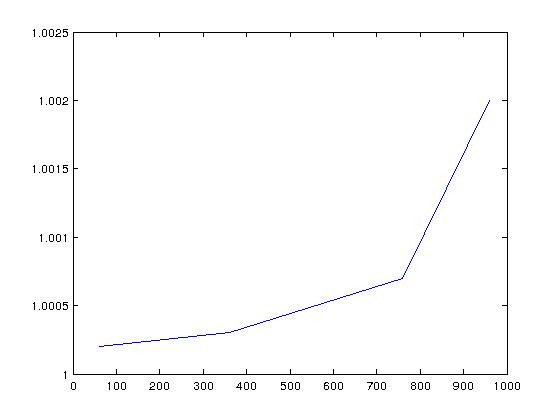
\includegraphics[scale=0.25]{Dim_MOR}
\caption{MOR vs Dimension}
\end{figure}

\begin{figure}[h]
\centering
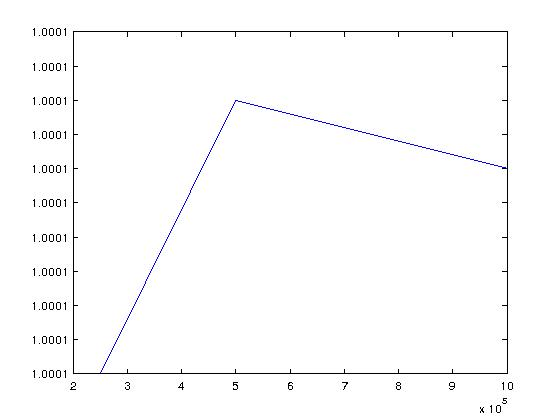
\includegraphics[scale=0.25]{SIze_MOR}
\caption{MOR vs Size}
\end{figure}

\begin{figure}[h]
\centering
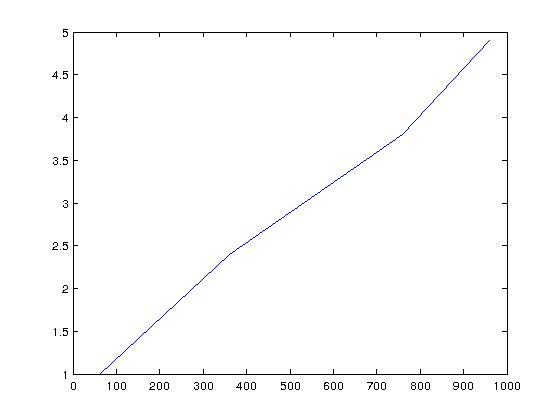
\includegraphics[scale=0.25]{Dim_Speed}
\caption{Query TIme vs Dimension}
\end{figure}


\begin{figure}[h]
\centering
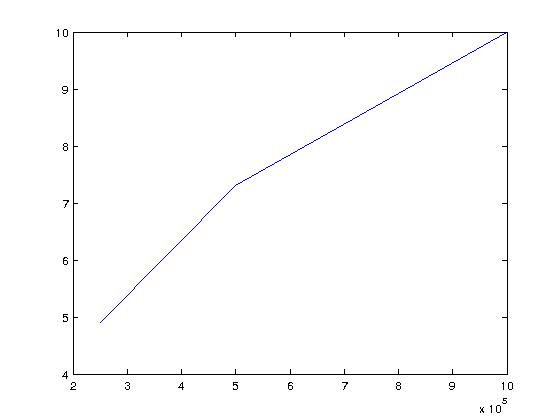
\includegraphics[scale=0.25]{size_speed}
\caption{Query TIme vs Size}
\end{figure}

\end{document}
